\documentclass[12pt]{article}
\usepackage[utf8]{inputenc}
\usepackage{geometry}
\usepackage{amsfonts}
\usepackage{hyperref}
\usepackage{enumitem}
\usepackage{graphicx}
\usepackage{tabularx}
\usepackage{amsmath}
\usepackage{xcolor}
\usepackage{array}
\usepackage{tikz}

\newcommand{\prob}[1]{\mathbb{P}\left[#1\right]}
\newcommand{\true}{\textsc{true}}
\newcommand{\false}{\textsc{false}}


\title{
    \textbf{CSE643: Artificial Intelligence} \\ \vspace*{-5pt}
    \textbf{\large{Assignment-3}}
}

\author{\href{mailto:divyajeet21529@iiitd.ac.in}{Divyajeet Singh (2021529)}}
\date{\today}

\geometry{a4paper, left=20mm, right=20mm, top=20mm, bottom=20mm}


\begin{document}
    \maketitle

    \section*{Theory}

    \subsection*{Problem-1}
    \subsubsection*{(i)}
    We identify the following random variables in the given sentences
    \begin{enumerate}
        \item $T$: a boolean RV indicating if the person travelled or not
        \item $D$: an RV indicating the type of disease the person caught (\textsc{corona}, \textsc{other}, \textsc{none})
        \item $S$: an RV indicating the severity of the disease (\textsc{mild}, \textsc{severe}, \textsc{none})
        \item $L$: a boolean RV indicating if the person died
    \end{enumerate}
    Using probability notation, the given sentences can be written as follows
    \begin{enumerate}[label=(\alph*)]
        \item $\prob{T = \true \wedge D \neq \textsc{none}} = 0.825$
        \item $\prob{D = \textsc{corona} \wedge S = \textsc{mild} \ | \ T = \true} = 0.15$ \\
              $\prob{D = \textsc{corona} \wedge S = \textsc{severe} \ | \ T = \true} = 0.22$
        \item $\prob{D = \textsc{other} \ | \ T = \true} = 0.485$
        \item $\prob{L = \true \wedge D = \textsc{other} \ | \ T = \true} = 0.24$
        \item $\prob{T = \false \wedge D = \textsc{corona} \wedge S = \textsc{severe}} = 0.025$
        \item $\prob{S = \textsc{severe} \ | \ T = \false} = 0.457$
        \item $\prob{L = \true \wedge D = \textsc{corona}} = 0.059$
        \item $\prob{S \neq \textsc{none}} = 0.7$
        \item $\prob{T = \true \ | \ S = \textsc{severe}} = 0.8$
        \item $\prob{D = \textsc{corona} \ | \ T = \true} = \prob{D = \textsc{corona} \ | \ T = \false} = 0.5$
    \end{enumerate}

    \subsubsection*{(ii)}
    Now, we verify that the above system satisfy probability axioms and from a valid distribution. We
    can infer from the above that
    \begin{enumerate}
        \item $\prob{D = \textsc{none} \ | \ T = \true} = 1 - 0.5 - 0.485 = 0.015$
        \item $\prob{D = \textsc{corona} \wedge S = \textsc{none} \ | \ T = \true} = 0.5 - 0.15 - 0.22 = 0.13$
    \end{enumerate}
    It is hence clear that the given problem forms a valid distribution. So, it follows the
    following conditional probability axioms
    \begin{enumerate}
        \item All conditional probabilities are non-negative and at most 1, i.e. $$0 \leq \prob{e \ | \ B} \leq 1 \quad \forall \ e \in B \subseteq S$$
        \item The sum of all conditional probabilities given condition is 1, i.e. $$\sum_{e \in B} \prob{e \ | \ B} = 1 \quad \forall \ B \subseteq S$$
        \item Bayes' Theorem, which states $$\prob{ A \ | \ B} = \frac{\prob{B \ | \ A} \prob{A}}{\prob{B}}, \quad \forall A, B \subseteq S$$
    \end{enumerate}

    \subsubsection*{(iii)}
    The joint probability distribution table is given in table \ref{tab:joint-prob}.
    \begin{table}[htbp]
        \centering
        \renewcommand{\arraystretch}{1.5}
        \begin{tabular}{cccc|c}
            $T$ & $D$ & $S$ & $L$ & $\prob{T = t \wedge D = d \wedge S = s \wedge L = l}$ \\
            \hline
            % $\true$ & \textsc{corona} & \textsc{mild} & $\true$ \\
            % $\true$ & \textsc{corona} & \textsc{mild} & $\false$ \\
            % $\true$ & \textsc{corona} & \textsc{severe} & $\true$ \\
            % $\true$ & \textsc{corona} & \textsc{severe} & $\false$ \\
            % $\true$ & \textsc{other} & \textsc{mild} & $\true$ \\
            % $\true$ & \textsc{other} & \textsc{mild} & $\false$ \\
            % $\true$ & \textsc{other} & \textsc{severe} & $\true$ \\
            % $\true$ & \textsc{other} & \textsc{severe} & $\false$ \\
            % $\true$ & \textsc{none} & \textsc{mild} & $\true$ \\
            % $\true$ & \textsc{none} & \textsc{mild} & $\false$ \\
            % $\true$ & \textsc{none} & \textsc{severe} & $\true$ \\
            % $\true$ & \textsc{none} & \textsc{severe} & $\false$ \\
            % $\false$ & \textsc{corona} & \textsc{mild} & $\true$ \\
            % $\false$ & \textsc{corona} & \textsc{mild} & $\false$ \\
            % $\false$ & \textsc{corona} & \textsc{severe} & $\true$ \\
            % $\false$ & \textsc{corona} & \textsc{severe} & $\false$ \\
            % $\false$ & \textsc{other} & \textsc{mild} & $\true$ \\
            % $\false$ & \textsc{other} & \textsc{mild} & $\false$ \\
            % $\false$ & \textsc{other} & \textsc{severe} & $\true$ \\
            % $\false$ & \textsc{other} & \textsc{severe} & $\false$ \\
            % $\false$ & \textsc{none} & \textsc{mild} & $\true$ \\
            % $\false$ & \textsc{none} & \textsc{mild} & $\false$ \\
            % $\false$ & \textsc{none} & \textsc{severe} & $\true$ \\
            % $\false$ & \textsc{none} & \textsc{severe} & $\false$ \\
        \end{tabular}
        \caption{Joint Probability Distribution Table}
        \label{tab:joint-prob}
    \end{table}

    \subsubsection*{(iv)}
    It is clear that all variables are conditionally dependent on each other.

    \subsection*{Problem-3}
    We know apriori that the key is behind one of the three doors. If we choose a door
    that does not have the key, we lose a life.

    \subsubsection*{(a)}
    Apriori, with no other information, the probability that the key is behind any
    door is $\frac{1}{3}$. Let $K$ be the random variable indicating the door behind
    which the key is. Then,
    \begin{equation}
        \prob{K = i} = \frac{1}{3} \implies \prob{K \neq i} = 1 - \frac{1}{3} = \frac{2}{3} \quad \forall \ i \in \{ 1, 2, 3 \}
    \end{equation}
    Without loss of generality, let us assume that we picked door 1, and the adversary
    who knows where the key is, opens door 2. There are clearly only three possible cases,
    which are listed in table \ref{tab:cases}. Clearly, the probability of winning the key
    is $\frac{1}{3}$ if we stick to our choice and $\frac{2}{3}$ if we switch. Hence,
    \textbf{the optimal strategy is to switch}.
    \begin{table}[htbp]
        \centering
        \renewcommand{\arraystretch}{1.5}
        \begin{tabular}{c|cc}
            \textsc{Random-variable} & \textsc{Stick} & \textsc{Switch} \\
            \hline
            $K = 1$ & \texttt{Win the key} & \texttt{Lose a life} \\
            $K = 2$ & \texttt{Lose a life} & \texttt{Win the key} \\
            $K = 3$ & \texttt{Lose a life} & \texttt{Win the key} \\
        \end{tabular}
        \caption{Possible cases in the escape room puzzle}
        \label{tab:cases}
    \end{table}
    \vspace*{0pt} \\
    Intuitively, switching is more likely to land on a door with the key because
    you are more likely to pick an empty door in the first place. So, when the
    adversary reveals another empty door, it is \textit{more} likely that the
    key is behind the third door.

    \subsubsection*{(b)}
    Now, we are given that the adversary can sometimes makes a mistake. So, we get the following
    sequence of events.
    \begin{center}
        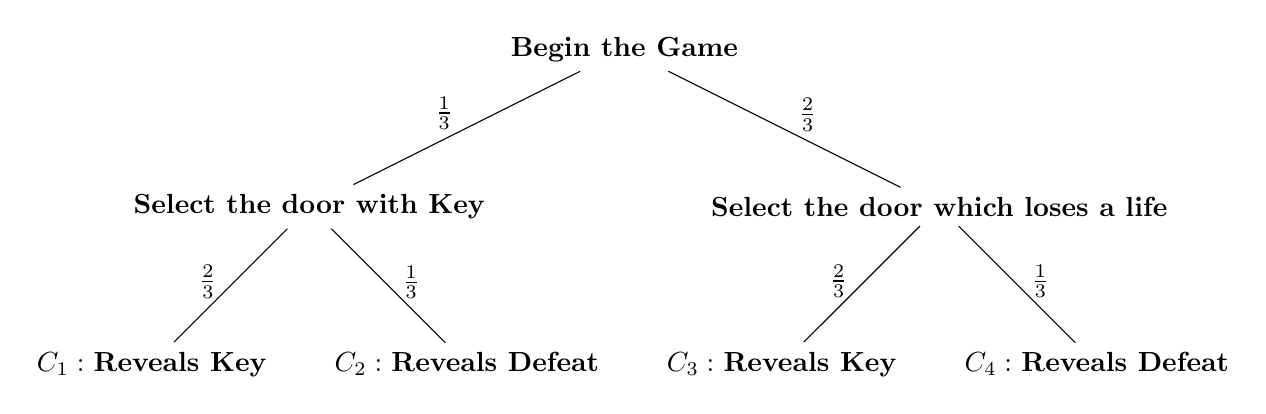
\begin{tikzpicture}
            [level/.style={sibling distance=45mm/#1},
            every node/.style={rectangle, align=center},
            level 1/.style={sibling distance=80mm},
            level 2/.style={sibling distance=40mm},
            level distance=20mm]

            \node {\textbf{Begin the Game}}
            child {
                node {\textbf{Select the door with Key}}
                child {
                    node {$C_{1}:$ \textbf{Reveals Key}}
                    edge from parent node[midway, above, pos=0.7] {$\frac{2}{3}$}
                }
                child {
                    node {$C_{2}:$ \textbf{Reveals Defeat}}
                    edge from parent node[midway, above, pos=0.7] {$\frac{1}{3}$}
                }
                edge from parent node[midway, above, pos=0.6] {$\frac{1}{3}$}
            }
            child {
                node {\textbf{Select the door which loses a life}}
                child {
                    node {$C_{3}:$ \textbf{Reveals Key}}
                    edge from parent node[midway, above, pos=0.7] {$\frac{2}{3}$}
                }
                child {
                    node {$C_{4}:$ \textbf{Reveals Defeat}}
                    edge from parent node[midway, above, pos=0.7] {$\frac{1}{3}$}
                }
                edge from parent node[midway, above, pos=0.6] {$\frac{2}{3}$}
            };
        \end{tikzpicture}
    \end{center}
    where "Defeat" means the loss of a life. We can now calculate the probability of winning
    the key if we stick to our choice and if we switch. For this, we assume that no matter what,
    the adversary will always follow the given probabilities to select a door to open (i.e., the
    man might open the door we pick in case it has the key).
    We now look at each case
    \begin{enumerate}
        \item \textbf{Case-1}: We picked the door with the key and the adversary reveals the key. In
        this case, we win the key if we stick to our choice.
        \item \textbf{Case-2}: We picked the door with the key and the adversary reveals defeat. In this
        case, we should ideally stick to our choice.
        \item \textbf{Case-3}: We picked the door without the key and the adversary reveals the key. In this
        case, we lose anyway. So, let's assume switching is better.
        \item \textbf{Case-4}: We picked the door without the key and the adversary reveals defeat. In this
        case, we should switch, since this is equivalent to the original problem.
    \end{enumerate}
    So, we get the following table of probabilities.
    \begin{table}[htbp]
        \centering
        \renewcommand{\arraystretch}{1.5}
        \begin{tabular}{c|c|cc}
            \textsc{Case} & \textsc{Probability} & \textsc{Stick} & \textsc{Switch} \\
            \hline
            $C_{1}$ & $\frac{1}{3} \cdot \frac{2}{3} = \frac{2}{9}$ & \texttt{Win the key} & \texttt{Lose a life} \\
            $C_{2}$ & $\frac{1}{3} \cdot \frac{1}{3} = \frac{1}{9}$ & \texttt{Win the key} & \texttt{Lose a life} \\
            $C_{3}$ & $\frac{2}{3} \cdot \frac{2}{3} = \frac{4}{9}$ & \texttt{Lose a life} & \texttt{Lost the game} \\
            $C_{4}$ & $\frac{2}{3} \cdot \frac{1}{3} = \frac{2}{9}$ & \texttt{Lose a life} & \texttt{Win the key} \\
        \end{tabular}
        \caption{Possible cases in the escape room puzzle with mistakes}
        \label{tab:mistake-cases}
    \end{table}
    \vspace*{0pt} \\
    So, the probability of winning the key if we stick to our choice is $\frac{3}{9}$, and
    the probability of winning the key if we switch\footnote{
        Here, we assume that we cannot switch to the open door, which contains the key. Hence,
        on switching, the chances of losing increase. Case $C_{3}$ happens with probability
        $\frac{4}{9}$, which is a destined loss.
    } is $\frac{2}{9}$. Hence, \textbf{the optimal
    strategy is to stick}.

    \subsubsection*{(c)}
    Here, we choose to swtich. We need to find the conditional probability of winning the key given that
    the man/adversary has revealed the door that shows the loss of a life. Let the random variable
    $W$ indicate if we selected the winning door or not. Then, we are interested in the probability
    \begin{align}
        \prob{W = \true \ | \ C_{2} \vee C_{4}} &= \frac{\prob{W = \true \wedge (C_{2} \vee C_{4})}}{\prob{C_{2} \vee C_{4}}} \\
        &= \frac{\prob{W = \true \wedge C_{4}}}{\prob{C_{2}} + \prob{C_{4}}} \\
        &= \frac{\prob{W = \true} \cdot \prob{C_{4}}}{\prob{C_{2}} + \prob{C_{4}}} \\
        &= \frac{\frac{1}{3} \cdot \left( \frac{2}{3} \cdot \frac{1}{3} \right)}{\frac{1}{3} \cdot \frac{1}{3} + \frac{2}{3} \cdot \frac{1}{3}} = \frac{2}{9}
    \end{align}
    Where the second equality follows because if we win by switching, then $C_{2}$ is impossible, and the
    third equality follows by the independence of the player picking a door and the person picking the door to reveal.

    \subsubsection*{(d)}
    Let us assume that the reward $R$ for winning the key is 1 and losing a life is -1. Then, the expected
    reward is
    \begin{align}
        \mathbb{E}[R \ | \ \texttt{Switch}] &= \prob{W = \true \ | \ C_{2} \vee C_{4}} \cdot 1 + \prob{W = \false \ | \ C_{2} \vee C_{4}} \cdot (-1) \\
        &= \frac{2}{9} \cdot 1 + \frac{7}{9} \cdot (-1) = -\frac{5}{9} \approx -0.555
    \end{align}
    We now find the probability of winning if we choose to stick.
    \begin{align}
        \prob{W \ | \ \texttt{Stick}} &= \prob{W = \true \wedge (C_{1} \vee C_{2})} \\
        &= \prob{W = \true \wedge C_{1}} + \prob{W = \true \wedge C_{2}} \\
        &= \frac{1}{3} \cdot \frac{2}{3} + \frac{1}{3} \cdot \frac{1}{3} = \frac{1}{3}
    \end{align}
    So, we have
    \begin{align}
        \mathbb{E}[R \ | \ \texttt{Stick}] &= \prob{W = \true \ | \ C_{1} \vee C_{2}} \cdot 1 + \prob{W = \false \ | \ C_{1} \vee C_{2}} \cdot (-1) \\
        &= \frac{1}{3} \cdot 1 + \frac{2}{3} \cdot (-1) = -\frac{1}{3} \approx -0.333
    \end{align}
    So, the expected reward for switching is -0.555, and for sticking is -0.333. Hence, \textbf{the optimal
    strategy is to stick}.

    \section*{Computational}
    The solution to the computational part of the assignment is given in the code in \texttt{main.ipynb} in the submission.
    The code uses the \texttt{bnlearn} package in Python to implement Bayesian Networks.
    The constructed Bayesian Network is used in prediction of the target variable in
    the Wine Quality Dataset provided on the UCI-ML Repo.

    \section*{References}
    \begin{enumerate}
        \item \href{https://erdogant.github.io/bnlearn/pages/html/index.html}{\color{blue}\underline{BNLearn Official Documentation}}
    \end{enumerate}

\end{document}